\documentclass{beamer}
\usepackage[utf8]{inputenc}
\usepackage[romanian]{babel}
\usepackage{hyperref}
\usepackage{mathtools}
\usepackage{listings}
\usepackage{graphicx}
\usepackage{float}
\usepackage{xcolor}
\usepackage{adjustbox}
\usepackage{scalerel}
\usepackage{tikz}
\usetikzlibrary{arrows}
\usetikzlibrary{calc}
\usepackage{pgfplots}

\date{}

\setbeamercovered{transparent}
\usetheme{Madrid}
\title{Traffic Manager}
\author{Student: Mihai Andrei Gherghinescu \\ Supervizor: Lect. Dr. Todor Ivașcu}

\graphicspath{ {./images/} }

\begin{document}

\frame{\titlepage}

\section{Introducere}
    \begin{frame}{Introducere}
        Una dintre principalele cauze ale congestiilor in trafic
        sunt intersectiile. Pentru a minimiza timpul pierdut atat cat si siguranta soferilor 
        au fost dezvoltate sisteme de trafic inteligente(ITS). Urmeaza sa prezentam 
        un scurt istoric al tehnologiilor dezvoltate cat si sa propunem o noua abordare a 
        acestei probleme.
    \end{frame}

\section{Tehnologiei dezvoltate dealungul timpului}
    \begin{frame}{Tehnologiei dezvoltate dealungul timpului}
        \begin{itemize}[<+-| alert@+>]
            \item Sisteme bazate pe detectia de obiecte 
            \begin{itemize}
                \item Principiu de baza: detectia de masini pe baza imaginilor
                \item Dezavantaje: complexitate computationala mare; neeficiente in conditi neprielnice de mediu
            \end{itemize}
            \item Sisteme bazate pe senzori
            \begin{itemize}
                \item Principiu de baza: detectie de masini pe baza senzorilor
                \item Dezavantaje: costuri mari
            \end{itemize}
            \item Sisteme care sincronizeaza traficul
            \begin{itemize}
                \item Principiu de baza: minimizarea numarului de opriri/porniri in trafic
                \item Dezavantaje: presupune viteza constanta in trafic a autovehiculelor; ineficiente cand doua sau mai multe
                rute principale se intersecteaza
            \end{itemize}
            \item Sisteme bazate pe logica fuzzy
            \begin{itemize}
                \item Principiu de baza: aproximarea stari traficului utilizand seturi fuzzy de valori ale lungimi luminii verzi a semaforului
                \item Dezavantaje: training real-time de durata mare, posibilitatea ingreunari traficului
            \end{itemize}
            \item Sisteme bazate pe DSRC
            \begin{itemize}
                \item Principiu de baza: folosirea de semnale radio specializate pentru a determina starea traficului
                \item Dezavantaje: infrastructura nu permite lansarea acestor tipuri de sistem
            \end{itemize}
        \end{itemize}
    \end{frame}


\section{Motivatie, scopuri si obiective}
    \begin{frame}{Motivatie, scopuri si obiective}

        \begin{itemize}[<+-| alert@+>]
        \item Motivatie: ambuteiajele frecvente in trafic in timpul orelor de varf/
        conditii neasteptate de trafic, cand majoritatea sistemelor dezvoltate pana acum esueaza
        \item Obiective ale sistemului:
            \begin{itemize}
                \item Performant si accesibil
                \item Adaptabil la orice conditie de trafic
                \item Scalabil la nivel global 
            \end{itemize}
        \end{itemize}
    \end{frame}

\section{O noua varianta flexibila si economica de a gestiona traficul}
    \begin{frame}{O noua varianta flexibila si economica de a gestiona traficul}
        Credem că viitorul gestionari traficului se va baza pe semnale
        asemanatoare cu cele DSRC asa ca dorim sa oferim o migrare ușoară la 
        acest tip de tehnologie. Pentru asta am conceput un sistem IPC 
        alcatuit din 2 tipuri de servere si 2 tipuri de clienti:
        \begin{itemize}[<+-| alert@+>]
            \item Clienti:
            \begin{enumerate}
                \item Traffic Observer(TO) - legat de catre o camera pe fiecare directie
                \item Vehicle Tracker(VT) - instalat direct pe autovehicul
            \end{enumerate}
            \item Servere: 
            \begin{enumerate}
                \item  Proxy - servere regionale ce asigura conectivitatea
                \item  Junction Main Server(JMS) - legat de intersectie si semafoare
            \end{enumerate}
        \end{itemize}

    \end{frame}

    \begin{frame}{Junction main server}
        \begin{figure}[h!]
            \includegraphics[width=\textwidth]{Sketches/AvailableJunctionphases.png}
            \caption{Fazele traficului}
            \label{fig:Junction_phases}
        \end{figure}

    \end{frame}

    \begin{frame}{Junction main server}
        \begin{figure}[h!]
            \includegraphics[width=\textwidth]{Sketches/SwitchingTroughphasesExample.png}
            \caption{Exemplu flow al traficului}
            \label{fig:phasesSwitchingExample}
        \end{figure}
        
    
    \end{frame}
    \begin{frame}{Junction main server}
        
        \begin{figure}[h!]
            \includegraphics[width=\textwidth]{Sketches/phaseSwitchingCaseToBeAvoided.png}
            \caption{Scenariu de conflict}
            \label{fig:FaultyphaseSwitching}
        \end{figure}

    \end{frame}

\section{Detalii de implementare}
    \begin{frame}{Detalii de implementare}
        Întregul sistem a fost dezvoltat folosind C++17, Python, Boost, OpenSSL, GLFW,
        MSVC WinAPI, OpenCV, Tensorflow, YoloV8 și MySQL. Sistemul în sine este
        tratat ca un proiect mare și împărțit în mai multe submodule: 

    \begin{itemize}
        \item librari
        \begin{itemize}
            \item Common
            \item CarDetector
            \item IPC
            \item GUIGLFW
        \end{itemize}
        
        \item executabile
        \begin{itemize}
            \item servere
            \begin{itemize}
                \item Proxy
                \item JunctionMainServer
                \item ObjectDetectionServer
            \end{itemize}
            \item  clienti
            \begin{itemize}
                \item VehicleTracker
                \item TrafficObserver
            \end{itemize}
            \item mediu de testare
        \end{itemize}
    \end{itemize}
    \end{frame}

    \begin{frame}{Common}
        Ideea principală a submodulului Common este să acționeze ca o
        bibliotecă ajutatoare. Oferă soluții la următoarele
        probleme frecvent întâlnite precum:
        \begin{itemize}
            \item Probleme de concurenta
            \item Parsarea datele produse de GPS 
            \item Interactiuni cu baza de date
            \item Parsarea fisierelor de configurare
            \item Crearea unor actiuni planificate
            \item Logarea sincrona in scenarii multifir de executie
        \end{itemize}
    \end{frame}

    \begin{frame}{IPC}
        Pentru a stabili comunicarea între toate executabilele, un sistem IPC nou
        a fost dezvoltat, ce se foloseste de Boost Asio pentru operatiile cu socket-uri.
        Obiecte ale framework-ului:
        \begin{itemize}[<+-| alert@+>]
            \item Client
            \item Server
            \item Conexiune
            \item Mesaje
        \end{itemize}

    \end{frame}
    \begin{frame}{GUIGLFW}
        \begin{figure}[h!]
            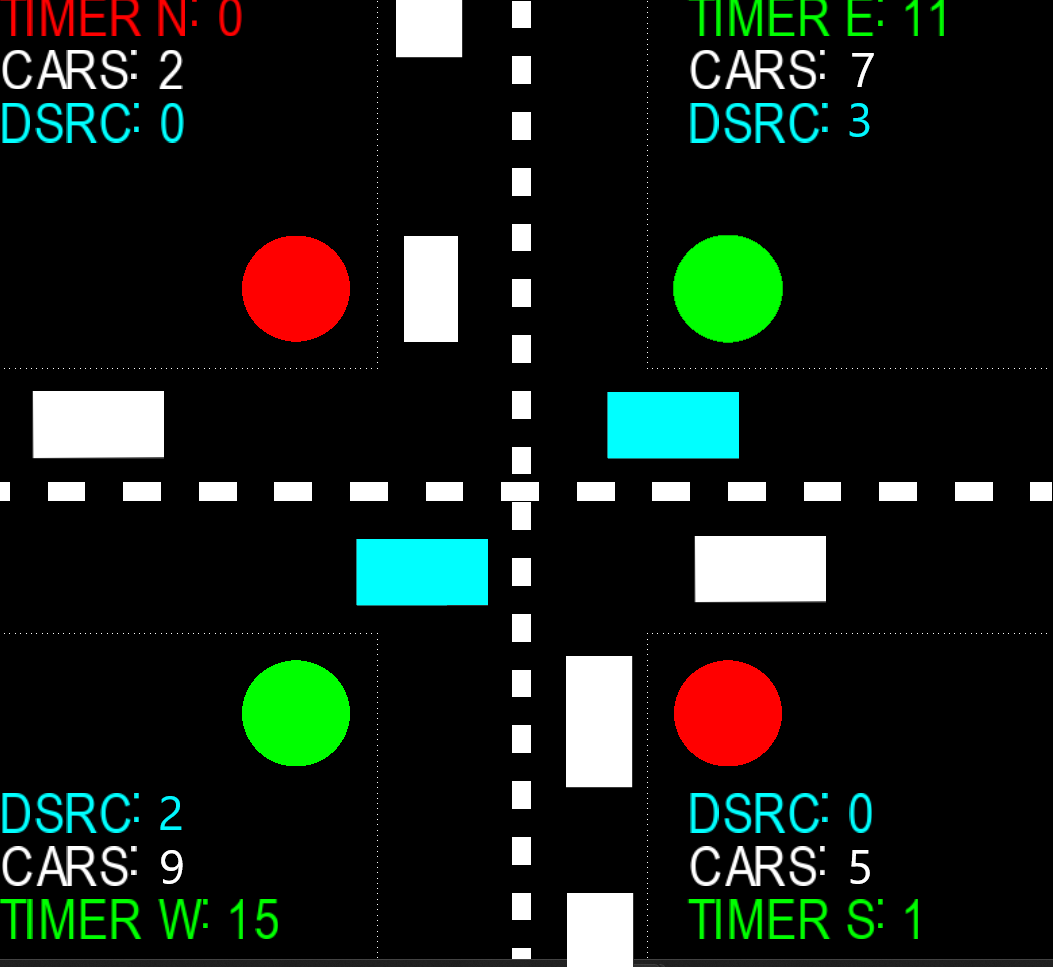
\includegraphics[width=(\textwidth / 3) * 2]{running/GUI_JMS.png}
            \caption{GUI JMS}
            \label{fig:GUI JMS}
        \end{figure}

    \end{frame}
    \begin{frame}{Car Detector}
        Detectia de masini se face in 2 etape:
        \begin{itemize}[<+-| alert@+>]
            \item detectia de obiecte in miscare folosind OpenCV
            \item determinarea daca acestea sunt sau nu masini folosing Tenserflow
            \item aproximarea urmatoarei pozitii si mentinerea unei evidente asupra acestora
        \end{itemize}
    \end{frame}

    \begin{frame}{Object Detection Server}
        Pentru a putea detecta dacă sunt prezente mașini, am încercat
        să utilizăm două arhitecturi diferite: una bazată pe YOLOv8 și
        una utilizând API-ul de detecție a obiectelor TensorFlow, în
        timp ce am folosit același set de date pentru antrenament.
        In urma unei analize indelungate, ce poate fi regasita in lucrare, 
        am determinat ca modelul antrenat folosind Tenserflow este mult 
        mai potrivit pentru scenariul nostru. Am folosit SSD MobileNet, un 
        tip de retea neuronala convolutionara ce a fost preantrenata si 
        este folosita deseori pe sisteme cu resurse limitate. Acuratetea medie 
        a modelului antrenat de noi este de 60\%, iar acesta este incarcat de 
        catre un server simplist scris in Python.
    \end{frame}

    \begin{frame}{Proxy}
        \begin{figure}[h!]
            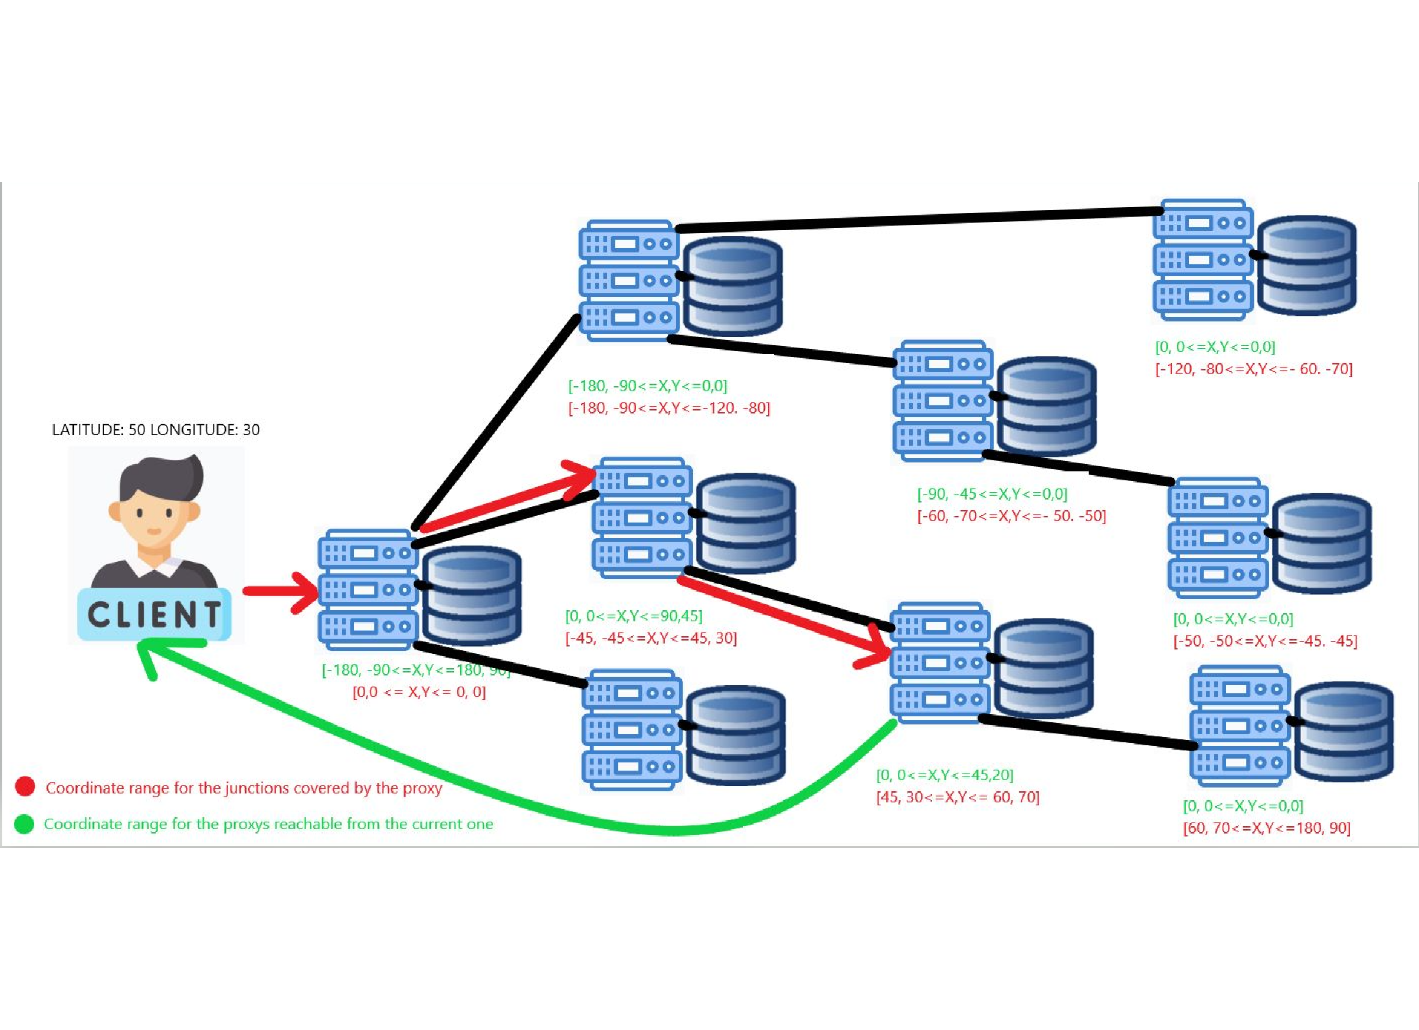
\includegraphics[width=(\textwidth / 6) * 5]{Sketches/ProxyFlowV2.png}
            \caption{Flow-ul de interogare a proxy-urilor}
            \label{fig:Proxy querys flow}
        \end{figure}
    \end{frame}


    \begin{frame}{JunctionMainServer}
        Implementarea în sine este concepută ca un state machine, 
        în care stările sunt reprezentate de stările traficului,
        iar evenimentele sunt reprezentate de expirarea cronometrelor.
        Fiecare stare are asociat un cronometru care scade în mod
        normal sau când este detectat un vehicul care urmeaza sa treaca
        prin intersectie. Ori de câte ori ne aflăm într-o anumită stare,
        cronometrul corespunzător este oprit și apoi resetat, iar 
        durata acestuia este recalculata in functie de trafic.
    \end{frame}

    \begin{frame}{JunctionMainServer}
        \begin{figure}[h!]
            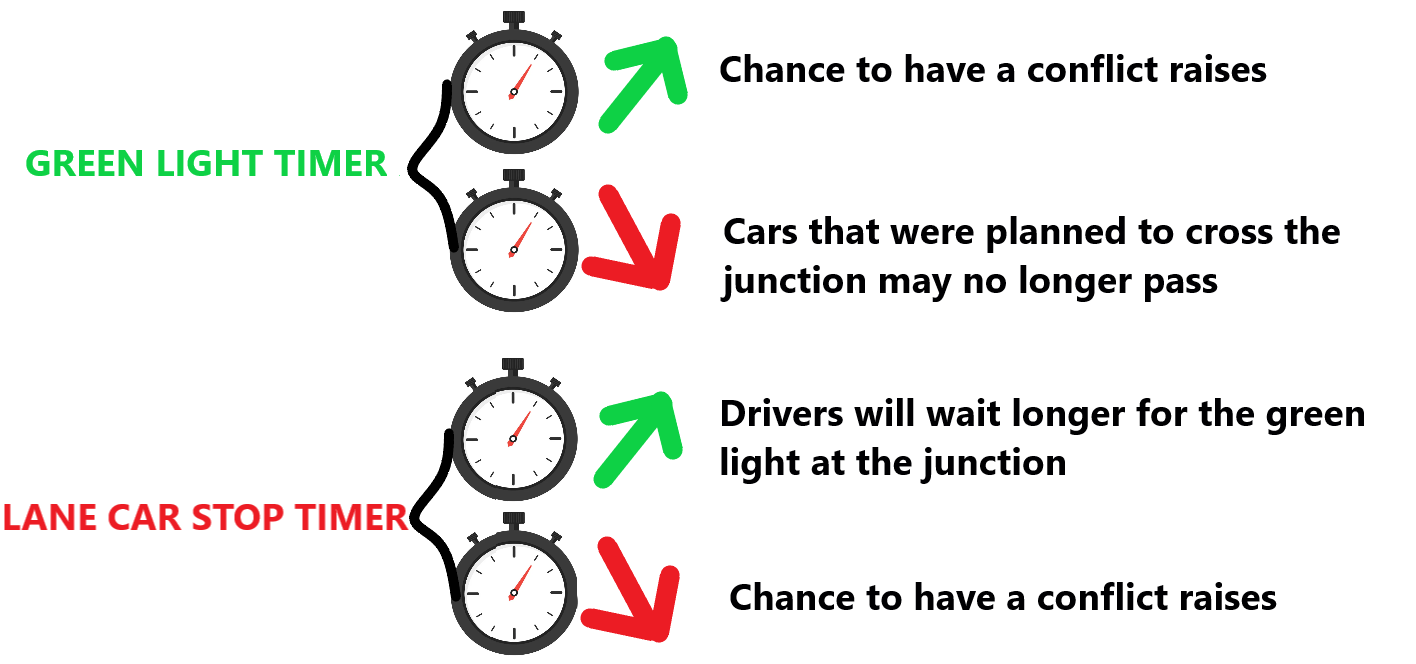
\includegraphics[width=\textwidth]{Sketches/TimerIncreaseDecreaseImpact.png}
            \caption{Impactul cresteri/scaderi durati cronometrului}
            \label{fig:Timer Increase/Decrease Impact}
        \end{figure}
    \end{frame}

    \begin{frame}{JunctionMainServer}
        Principiul de baza pe care incercam sa il obtinem este un timp 
        minim de astepare fara a intra in stari de conflict. Pentru 
        acest lucrur am retinut o medie a vehiculelor ce au trecut 
        de intersectie in timpul lumini verzi a semaforului si daca 
        suntem sau nu in stare de conflict.
    \end{frame}

    \begin{frame}{JunctionMainServer}    
        \begin{figure}[h!]
            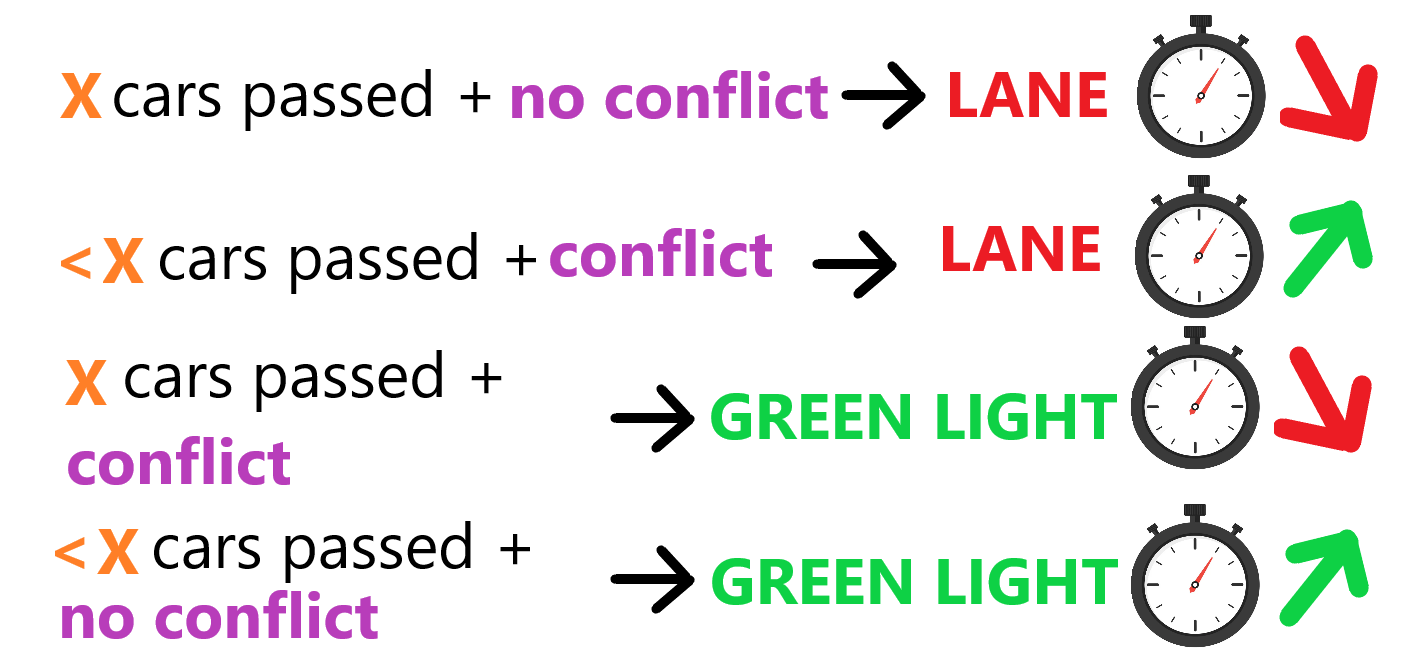
\includegraphics[width=\textwidth]{Sketches/FaultyScenariosHandling.png}
            \caption{Faulty Scenarios Handling}
            \label{fig:Faulty Scenarios Handling}
        \end{figure}
    \end{frame}

    \begin{frame}{TrafficObserver}
        \begin{figure}[h!]
            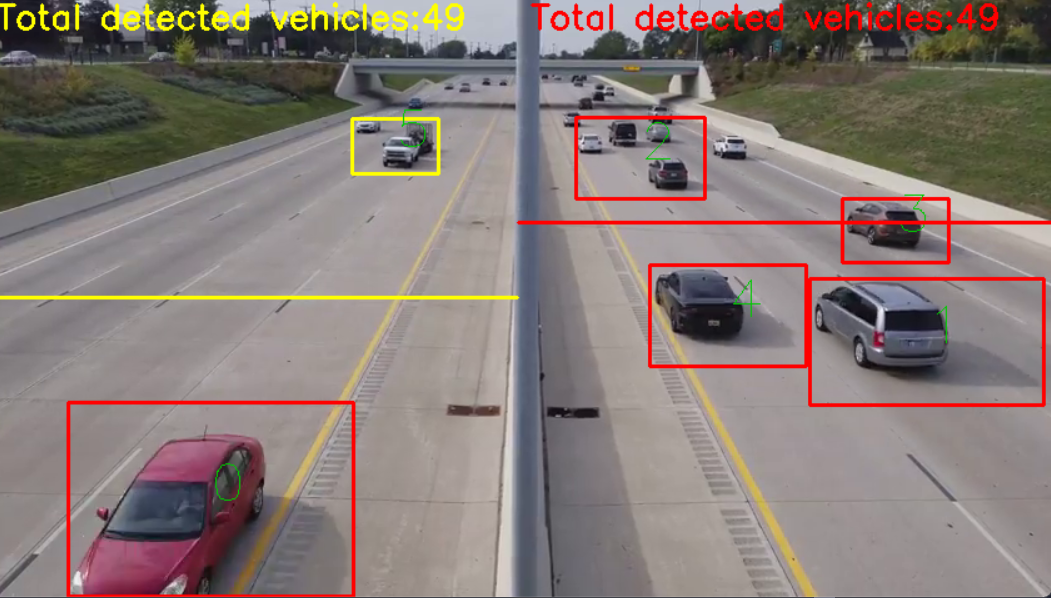
\includegraphics[width=\textwidth ]{TrafficDetectionRunningExample2.png}
            \caption{Exemplu detectie masini }
            \label{fig:Running client samples}
        \end{figure}

        
    \end{frame}

    \begin{frame}{VehicleTracker}

        \begin{itemize}[<+-| alert@+>]
            \item Se bazeaza pe prezenta unui GPS si parseaza date in format NMEA
            \item Interogheaza proxiul pentru a afla urmatoarea intersectie
            \item Se conecteaza la server-ul corespunzator intersectiei si asteapta pana cand trece de aceasta
            \item Se deconecteaza, si reia procesul, interogand ultimul proxi cunoscut
        \end{itemize}

    \end{frame}

    \begin{frame}{Mediu de testare}
        
        Pentru a putea testa întregul nostru sistem, am creat un
        executabil care să emuleze condițiile de trafic și să ruleze
        sistemul nostru. Executabilul primește mai multe fișiere de
        configurare ca intrare și poate rula simultan mai multe servere
        (JMS/Proxy-uri) și mai mulți clienți de orice tip, in orice fel 
        de combinatie. Pentru a emula mișcarea
        clienților instalati pe vehicule, am generat date GPS cu ajutorul
        \href{https://www.nmeagen.org/}{NMEAGEN}, iar pentru a simula
        inputul camerelor am colectat mai multe videoclipuri.

        LINK DEMO
    \end{frame}

\section{Concluzii, defecte ale sistemului si directii viitoare}
    \begin{frame}{Concluzii, defecte ale sistemului si directii viitoare}
        Am oferit o nouă modalitate alternativă de gestionare a traficului
        prin definirea și implementarea unui nou sistem de trafic,
        pe care credem că va îmbunătăți semnificativ traficul. Acesta 
        se poate adapta la conditiile de trafic, poate fi lansat la nivel global si 
        reprezinta o punte de trecere catre sistemele DSRC. De asemnea acesta 
        este accesibil deoarece nu necesita prezenta tuturor componentelor 
        hardware si/sau software pentru o buna functionare, iar majoritatea 
        cerintelor sunt deja indeplinite.
    \end{frame}

    \begin{frame}{Concluzii, defecte ale sistemului si directii viitoare}
        \begin{itemize}[<+-| alert@+>]
            \item Dificultati
            \begin{itemize}
                \item determinarea formulei de actualizare a duratei cronometrelor
                \item colectarea de date + simularea traficului
            \end{itemize} 
            \item Defecte ale sistemului
            \begin{itemize}
                \item potentialul unui atac cibernetic
                \item performanta afectata in cazul de conditii defavorabile de meteo
            \end{itemize}
            \item Directii viitoare
            \begin{itemize}
                \item un mecanism de "blacklisting" al atacatorilor
                \item mentinerea evidentei asupra masinilor la nivel geografic
                \item folosirea/crearea unui nou set de date bazat pe imagini radio
                \item imbunatatirea modelului de detectie al masinilor 
            \end{itemize}
        \end{itemize}
    \end{frame}

\end{document}